We test the implemented shuffle algorithm by measuring the throughput for varying dimensions of the CUDA grid and thread blocks. As a test setup we use two compute nodes connected by a 100Gb/s Infiniband interconnect. On each node one PE is executed using a NVIDIA V100 GPU. Our setup tests the performance of the shuffle for intra-node communication. Configurations that use both scale-up interconnects on the nodes and scale-out interconnects between the nodes introduce additional behavioural complexity that make it harder to evaluate the effects that are caused by NVSHMEM itself \cite{li2020}. Figure \ref{fig:shuffle_throughput} depicts the result of the shuffle benchmark.

\begin{figure}[h]
    \centering
    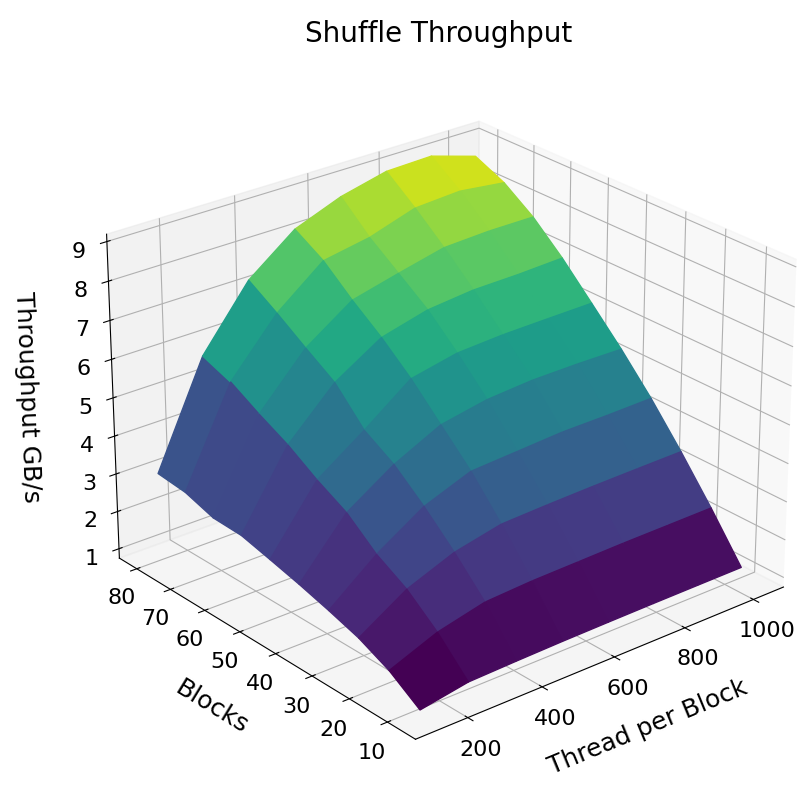
\includegraphics[width=0.6\textwidth]{img/shuffle_throughput.png}
    \caption{Throughput of shuffle algorithm for varying grid and block sizes}
    \label{fig:shuffle_throughput}
\end{figure}

The maximum throughput that can be reached using a high number of sending blocks is just under 9GB/s which would correspond to approximately 70\% of the link bandwidth. Recent work on parallelized CPU-driven shuffling operators using RDMA on the other hand has reported maximum throughput of slightly over 10GB/s \cite{liu2019}. To investigate the limiting factor of the shuffle we test the scanning and inserting of the tuples into the respective send buffers in isolation. Figure \ref{fig:atomic_insert} shows the result for this benchmark using the atomic increment insertion approach.  Notably the results are consistently higher than the link bandwidth. This suggests that the buffer sending introduces an overhead that leads to decreased performance. One aspect that influences the impact of sending on the performance is the correct behaviour of the asynchronous sending operations and intermediate synchronization to ensure buffers are ready for reuse before switching. To this end we conduct a test comparing the blocking send interface of NVSHMEM with the non-blocking asynchronous send interface with different synchronization strategies. As can be seen in Figure \ref{fig:block_nonblock} the execution time differences between the different approaches are negligible. This implies that actually the non-blocking operations do also block. We were not able to find an explanation for this divergence from the specified behaviour and can not make a conclusive statement on whether this is caused by our particular setup or a general problem of the library implementation. With the current implementation our shuffle implementation would directly benefit from correct non-blocking behaviour of the send interface. Based on this we can therefore hypothesize that correcting this error would likely improve our throughput performance.

\begin{figure}
    \centering
    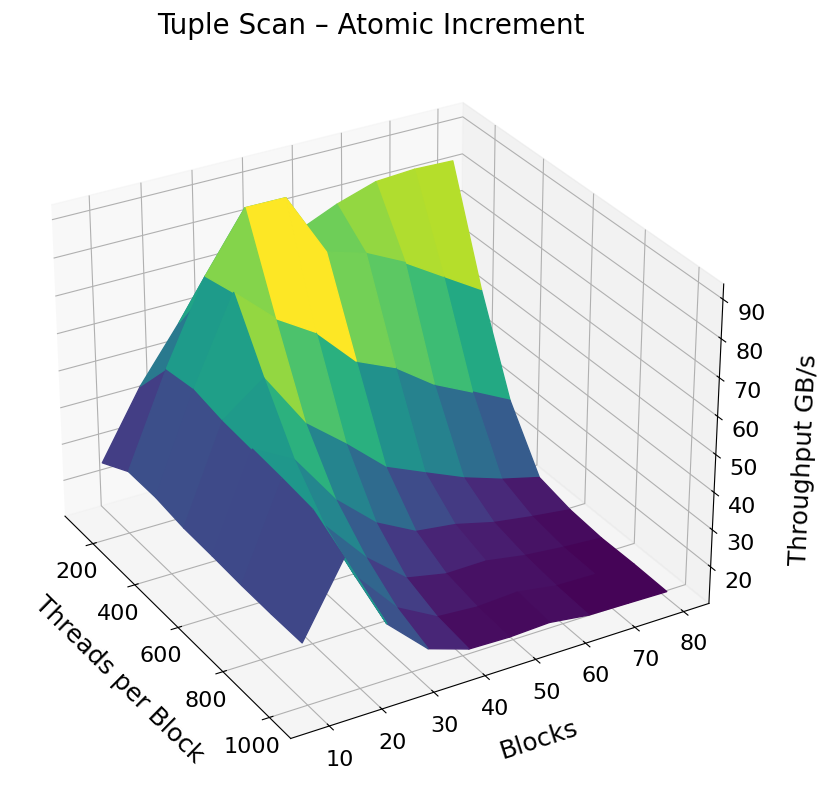
\includegraphics[width=0.6\textwidth]{img/scan_speed_atomic.png}
    \caption{Throughput of tuple scan and insertion using atomic increment as synchronization for varying numbers of blocks and threads}
    \label{fig:atomic_insert}
\end{figure}

\begin{figure}
    \centering
    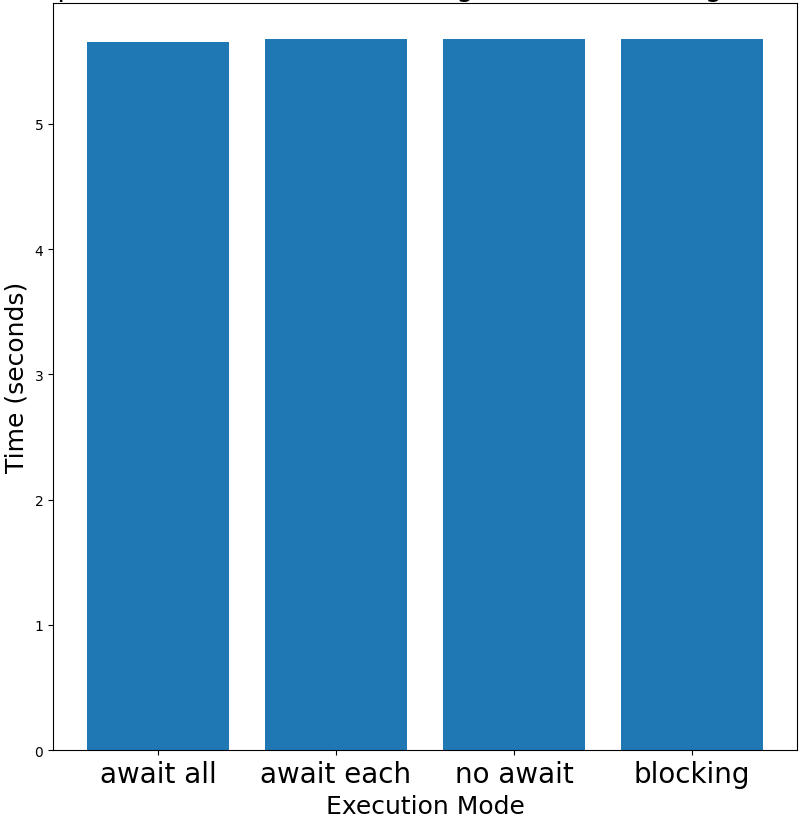
\includegraphics[width=0.4\textwidth]{img/blocking_nonblocking_barchart.png}
    \caption{Different approaches to non-blocking as well as blocking put operations showing the same behaviour}
    \label{fig:block_nonblock}
\end{figure}
